\section{Experiments}
\label{section:experiments}
[L'intro est ce necessaire ?]


First, we show on synthetic data that the proposed representation is identifiable provided that the hyperparameters and the reference graph are wisely selected, i.e.,
 the parameter $v_0^*$ generating a deformation $\varphi^{\{v_0^*\}}$ of a time series graph $\msg$ can be estimated from the data $\msg,\varphi^{\{v_0^*\}}.\msg$ by solving the geodesic shooting problem \eqref{eq:relaxation}.
 Secondly, we illustrate the qualitative interest of TS-LDDMM in studying inter-individual variability on a clinical dataset.
  Thirdly, we demonstrate the quantitative performance of our representation by performing classification on shape-based datasets.
  The method is implemented on Python using the library JAX\footnote{https://github.com/google/jax}. The code was compiled on a server with NVIDIA RTX A2000 12GB GPU, Intel(R) Xeon(R) Gold 5220R CPU @ 2.20GHz, and 250 GB of RAM. The code will be available on Github.
\subsection{Synthetic experiments}
\begin{figure}[t]
    \centering
    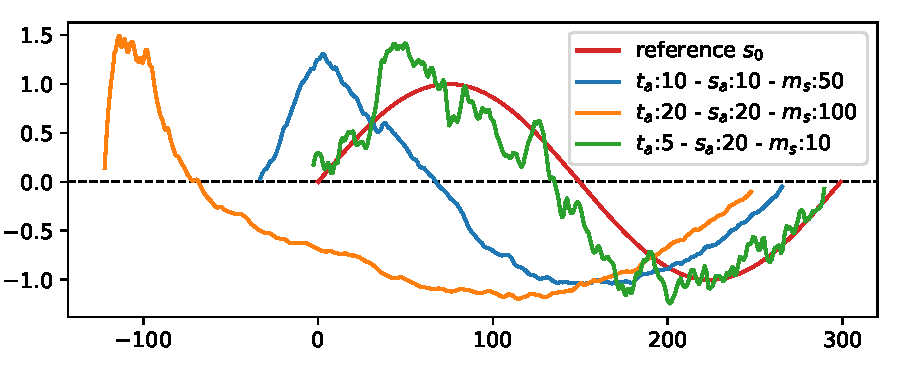
\includegraphics[width=0.5\linewidth]{pictures/samples.pdf}
    \vspace{-2.5em}
    \caption{Plots of $\varphi^{\{v_0(\mathbf{\alpha}^*,\msx)\}}.\msx$ for different values of $\mathbf{\alpha}^*$ according to its sampling parameter $t_a,s_a,m_s $, taking $\msx=\msg(s_0)$ with $s_0:k\in [300]\to \sin(2\pi k/300) $.}
    \label{fig:exemple_synthetic}
    \vspace{-1em}
\end{figure}

\begin{table}
    \caption{Values of $\scrl(\varphi^{\{v_0(\mathbf{\alpha}^*,\msx)\}}.\msx,\varphi^{\{\hat{v}_0\}}.\msx)$ as $\mathbf{\alpha}^*$ is sampled according to Gen(10,10,50) and $\hat{v}_0$ is estimated using $K_\msg$ with varying parameters $\sigma_{T,1},\sigma_x$.}
      \centering
         \begin{tabular}{lrrrrrrr}
         \toprule
         $\sigma_{T,0} \backslash \sigma_x$  & 1 & 10 & 50 & 100 & 200 & 300 \\
         \midrule
         0.1 & 2e+0 & 3e-4  & 1e-5&4e-6&7e-4&4e-3 \\
        1 & 4e-2 & 1e-4  & 1e-5&4e-6&7e-4 &4e-3  \\
         100 & 4e-2 & 2e-4  & 1e-5&4e-6&7e-4&4e-3  \\
         \bottomrule
         \end{tabular}
      \label{table:synthetic2}
      \vspace{-1em}
  \end{table}
 


% \begin{subfigure}{0.7\linewidth}
%   \centering
%   \resizebox{\columnwidth}{!}{%
%      \begin{tabular}{lrrrr}
%      \toprule
%      $\sigma_{T,0} \backslash \sigma_x$  & 0.1 & 1 & 100 \\
%      \midrule
%      1 & 2e+0 & 4e-2 & 4e-2 \\
%      10 & 3e-4 & 1e-4  & 2e-4 \\
%      50 & 1e-5 & 1e-5  & 1e-5 \\
%      100 & 4e-6 & 4e-6 & 4e-6 \\
%      200 & 7e-4 & 7e-4 & 7e-4 \\
%      300 & 4e-3 & 4e-3 & 4e-3 \\
%      \bottomrule
%      \end{tabular}
%      %
%      }
%  \caption{Values of $\scrl(y^*,\varphi^{\{\hat{v}_0\}}.\msx)$ where $y^*$ is sampled according to Gen(10,10,50) and $\hat{v}_0$ is estimated using $K_\msg$ with varying parameters $\sigma_{T,1},\sigma_x$.}
% \end{subfigure}
First, we show the model identifiability when the kernel $K_G$ is well specified: the estimated parameter is a good approximation of the generating parameter when the generation and the estimation procedure use the same hyperparameters for the RKHS kernel $K_\msg$.
All the hyperparameter values for generation and estimation are given in \Cref{appendix:numerics_synthetic}.
We fix the initial control points as $\msx=\left(x_k=(k,\sin(2\pi k/300))\right)_{k\in[300]} $.
Given $m_{s}\in \Nset_{>0}$ and $t_{a},s_{a}>0$, we randomly generate initial momentums $\mathbf{\alpha}^*=(\alpha_k^*)_{k\in[\mathbf{n}_0]}$ with the following sampling, called Gen($m_s,t_a,s_a$):
 For any $k\in[\mathbf{n}_0]$, $\mathbf{\alpha}_k'$ is sampled according to a Gaussian normal distribution $\mathcal{N}(0_{d+1},I_{d+1})$.
Then, $(\alpha_k')_{k\in[\mathbf{n}_0]}$ is regularized by a rolling average of size $m_{s}$, we get $\bar{\mathbf{\alpha}}'=(\bar{\alpha}_k')_{k\in[\mathbf{n}_0]}$.
Finally, we normalize $\bar{\mathbf{\alpha}}'$ to derive $\mathbf{\alpha}^*$ such that $|([\alpha_k^*]_t)_{k\in[\mathbf{n}_0]}|=t_{\text{amp}}$ and $|([\alpha_k^*]_s)_{k\in[\mathbf{n}_0]}|=s_{\text{amp}}$ for any $k\in[\mathbf{n}_0]$, denoting by $[\alpha_k^*]_t,[\alpha_k^*]_s$ the time and space coordinates of $\alpha_k^*$ respectively.
Note that the regularizing step $(\mathbf{\alpha}_k')_{k\in[\mathbf{n}_0]}\to \bar{\mathbf{\alpha}}' $ is necessary to obtain realistic deformations which take into account the regularity induced by the RKHS $\msv$.
%  uniformly on the set $\mss_M=\{ (\alpha_k)_{k\in[\mathbf{n}_0]}\in (\Rset^{d+1})^{\mathbf{n}_0}:\eqsp |\alpha_k|=M\}  $ with $M>0,\mathbf{n}_0\in \Nset_{>0}$,
%  then we regularize $\mathbf{\alpha}$ by convolving
%   with ... to get the generation parameter $\mathbf{\alpha}^*$.
Then, using $v_0(\mathbf{\alpha}^*,\msx)$ as defined in \eqref{eq:def_v0} with initial momentums $\mathbf{\alpha}^*$ and control points $\msx$, we apply the induced deformation $\varphi^{\{v_0\}} $ by \eqref{eq:integration} to $\msx$ and obtain $\varphi^{\{v_0\}}.\msx$.
Finally, we solve \eqref{eq:relaxation} to recover an estimation $\hat{\mathbf{\alpha}}$ of $\mathbf{\alpha}^*$ and report the average relative error (ARE) $|v_0(\hat{\mathbf{\alpha}},\msx)-v_0(\mathbf{\alpha}^*,\msx)|_\msv/|v_0(\mathbf{\alpha}^*,\msx)|_\msv$ on 50 repetitions.
This procedure is performed for any $m_{s},t_{a},s_{a}\in \{10,50,100\}\times \{5,10,15,20\}^2 $.
 Mean, standard deviation, and maximum of the ARE on all these hyperparameters choices are respectively $\mathbf{0.10, 0.03, 0.17}$.
 Therefore, the estimation procedure \eqref{eq:relaxation} offers a good approximation of the true parameter when the kernel $K_\msg$ is well specified.
 We observe that the estimation is difficult when $t_a\ll s_a$ because the time series can be very noisy as illustrated in \Cref{fig:exemple_synthetic}: this impacts the Varifold loss which is sensitive to tangents.
  
 Secondly, we demonstrate a weak identifiability when the kernel $K_\msg$ is misspecified: we can reconstruct the graph time series' after deformations even if the hyperparameters of $K_\msg$
  are different during the generation and the estimation.
   The hyperparameters of $K_\msg$ during generation are $(c_0,c_1,\sigma_{T,0},\sigma_{T,1},\sigma_x)=(1,0.1,100,1,1)$ and we fix $\sigma_{T,1},c_0,c_1=(1,1,0.1) $ for $K_\msg$ during estimation.
   We aim to understand the impact of $\sigma_{T,1},\sigma_x$ on the reconstruction since they are encoding the smoothness of the transformation according to time and space.  

    For any choice of the hyperparameters $\sigma_{T,1},\sigma_x\in \{1,10,50,100,200,300 \}\times \{0.1,1,100\}$ related to $K_\msg$ in the estimation,
     we average $\scrl(\varphi^{\{v_0(\mathbf{\alpha}^*,\msx)\}}.\msx,\varphi^{\{\hat{v}_0\}}.\msx)$ on 50 repetitions when $\mathbf{\alpha}^*$ is sampled according to Gen$(10,10,50)$ and $\hat{v}_0=v_0(\hat{\alpha},\msx)$ denoting by $\hat{\alpha}$ the result of the minimization \eqref{eq:relaxation}.
  We observe in \Cref{table:synthetic2} that the reconstruction is almost perfect except in the case when $\sigma_{t,0}=1$ during estimation, while $ \sigma_{t,0}=100$ during generation.
   Compared to $\sigma_{T,0}$, $\sigma_x$ has nearly no impact on the reconstruction.
   In \Cref{appendix:kernel_implementation}-\ref{appendix:kernel_TS_LDDMM}, we propose guidelines to drive future hyperparameters tuning and further discussions related to $\sigma_{T,1},c_0,c_1$. 
\subsection{Qualitative analysis of respiratory behavior in mice}
%We consider a dataset composed of mouse respiratory time series before and after a drug injection.
% A complete presentation of this dataset is given in \Cref{appendix:mouse_dataset}.
%  The mouse are divided in two groups depending on their genotypes : \textit{colq} and \textit{wt}.
%  We aim to study the difference of respiratory shapes according to the genotype.
%   That is why, TS-LDDMM \eqref{eq:general_optimization_problem} is applied to derive the features representations $(\mathbf{\alpha}_j)_{j\in[N]}\in (\Rset^2)^N$ related to $N$=\sam{fill} respiratory time series coming from 14 mouse (7 \textit{colq} and \textit{wt}) before drug injection.
%   Then, a Principal Components Analysis (PCA) is performed on $(\mathbf{\alpha}_j)_{j\in[N]}$
\begin{figure*}[t]
  \centering
  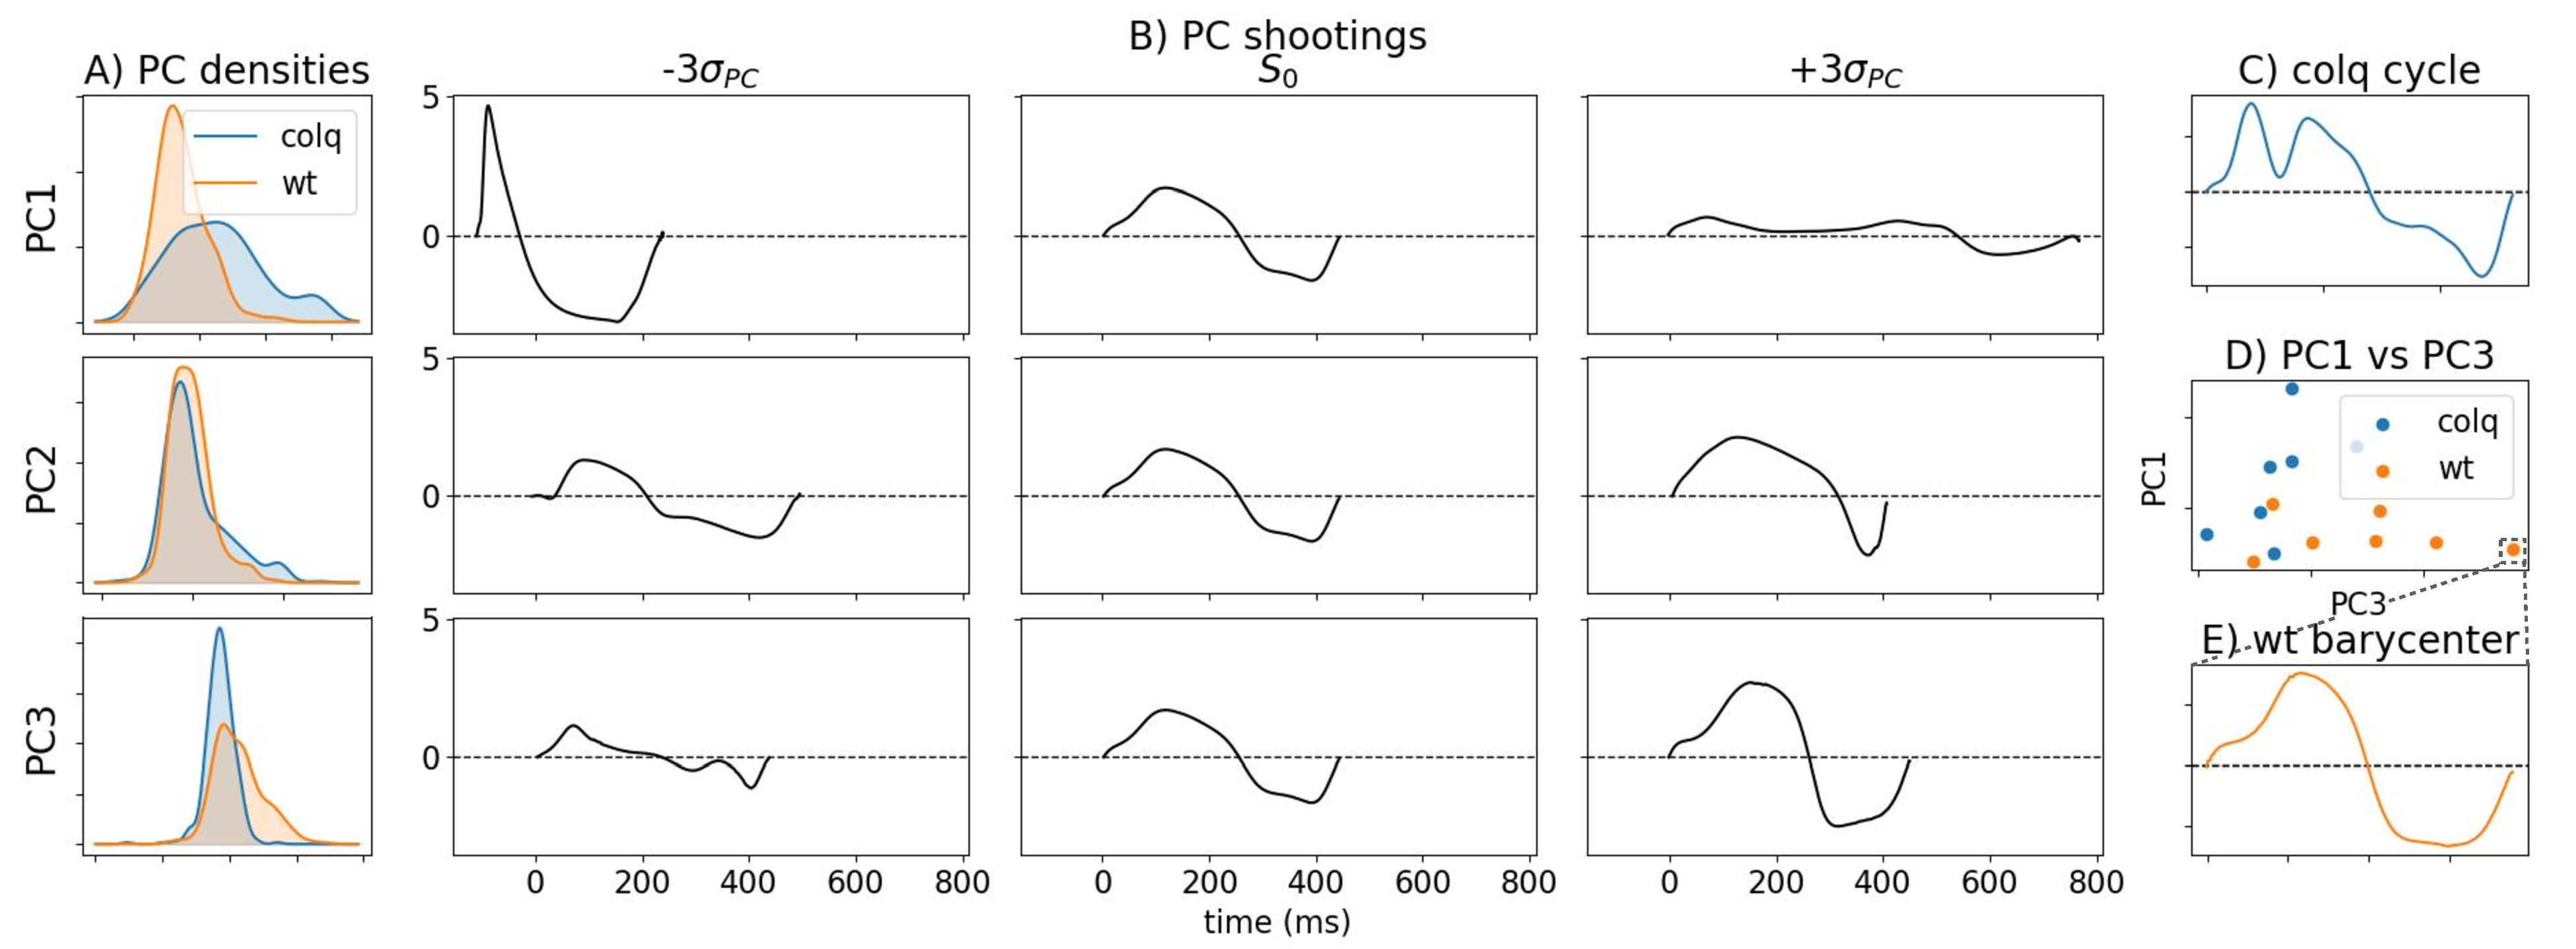
\includegraphics[width=0.95\linewidth]{"./pictures/exp_1_bis.pdf"}
  \vspace{-1.5em}
  \caption{Analysis of the three principal components (PC) related to the respiratory cycles of the mouse before exposure.
  In Figure A), the densities of each genotype according to each PC are displayed. In Figure B), the deformations of the reference graph $S_0$ along each PC are given. In Figure D), the graph of reference $S^j$, also called barycenter, related to each mouse, is displayed according to their coordinates on PC1 and PC3. In Figure C) et E), illustrations of respiratory cycles related to mice coming from the \textbf{wt} and \textbf{colq} group are displayed.  }
  \label{fig:exp_1_PCA}
  %\vspace{-1em}
\end{figure*}

\begin{figure*}[t]
  \centering
  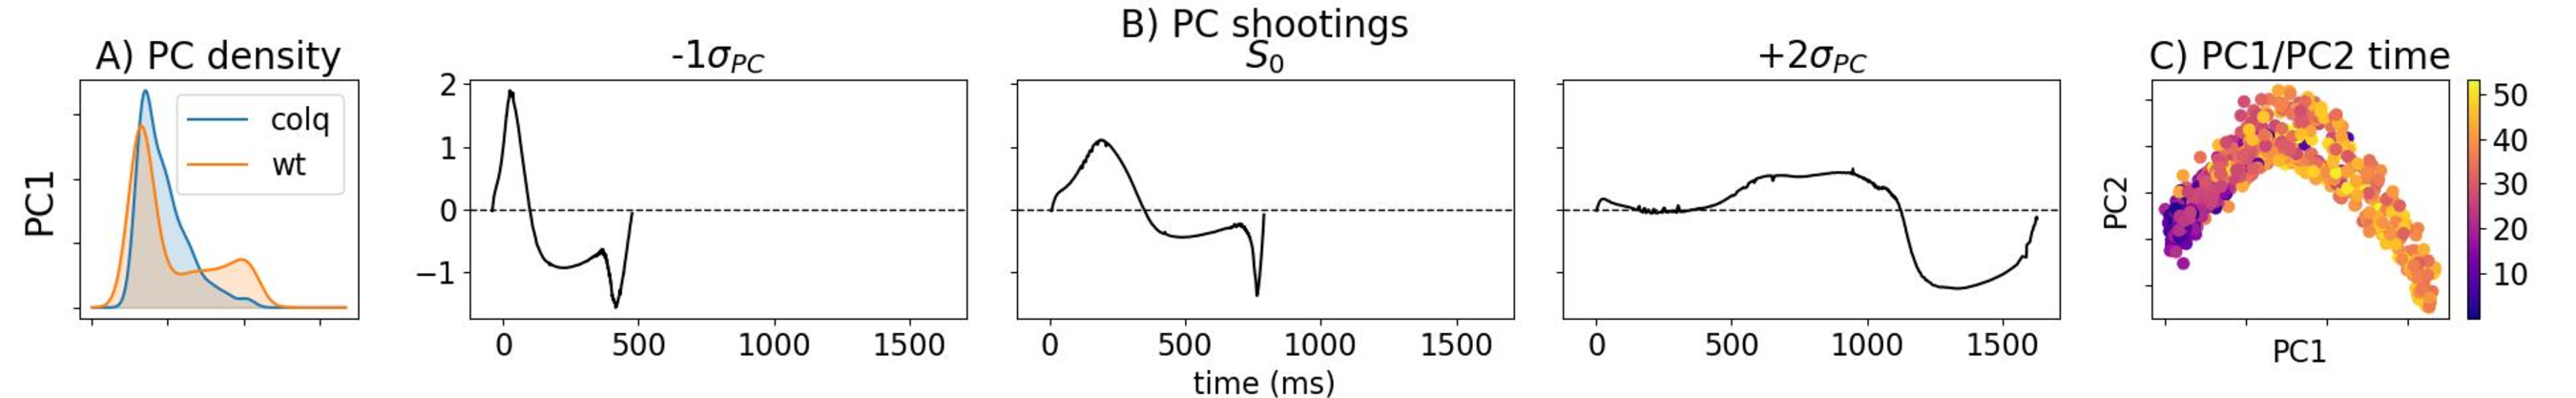
\includegraphics[width=0.95\linewidth]{"./pictures/exp_2.pdf"}
  \vspace{-1em}
  \caption{Analysis of the first Principal Component (PC1) related to the respiratory cycles of the mouse 
  before and after exposure. In Figure A), the densities of each genotype according are displayed. In Figure B), the deformations of the reference graph $S_0$ PC1 is given. In Figure C), respiratory cycles displayed with respect to time and according to their coordinates on PC1 and PC2}
  \label{fig:exp_2_PCA}
  \vspace{-1.5em}
\end{figure*}

This experiment highlights the \textit{interpretability} of TS-LDDMM for studying the inter-individual variability in a clinical dataset.
We consider a time series dataset recording the evolution of the respiratory airflow of mice exposed 
to an irritant molecule altering respiratory functions \cite{nervo2019respiratory}. The dataset is divided into two groups, one 
composed of 7 control mice (\textbf{wt}) and the other of 7 mice (\textbf{colq}) deficient in an enzyme 
involved in the control of respiration. For each mouse, the respiratory airflow was recorded for 
15 to 20 minutes before exposure to the irritant molecule and then for 35 to 40 minutes. A complete 
description of the dataset is given in the \Cref{appendix:mouse_dataset}.
By comparing the shape of individual respiratory cycles (inspiration + expiration, see \Cref{fig:exp_1_PCA}-C)), 
we show that TS-LDDMM features can encode genotype distinctive breathing behaviors and their evolution 
after exposure to the irritant molecule. 

We first compare breathing behaviors before exposure.
Solving \eqref{eq:general_optimization_problem}, we derive the reference respiratory cycle's graph $S_0$ and the TS-LDDMM features representations 
$(\alpha_j)_{j\in[N_1]}$ related to $N_1=700$ respiratory cycles extracted according 
to the procedure \cite{germain2023unsupervised}.
Then, we perform a kernel PCA on the initial velocity field $\left(v_0(\alpha_j,S_0)\right)_{j\in[N_1]}\in \msv^{N_1}$ defined in \eqref{eq:def_v0}.
In \Cref{fig:exp_1_PCA}, we focus on the analysis of the three Principal Components (PC).

As observable from \Cref{fig:exp_1_PCA}-B), principal components refer to different types of deformations. 
By interpreting \Cref{fig:exp_1_PCA}-B): Only PC1 accounts for time warping, PC2 expresses the trade-off between inspiration and expiration duration, and PC3 corresponds to a change in signal amplitude.
 Compared to \textbf{wt} mice, the distribution of \textbf{colq} mice 
TS-LDMMM feature representation along the PC1 axis has a heavy tail and the associated deformation (+3 $\sigma_{\text{PC}}$) 
shows an inspiration with two peaks. As illustrated in \Cref{fig:exp_1_PCA}-A), such respiratory cycles are preponderant
 with \textbf{colq} mice and may be caused by motor impairment due to their enzyme deficiency, \cite{germain2023unsupervised}.
  In addition, 
 the \textbf{colq} mice were smaller than the \textbf{wt} mice due to a delay in growth caused by their lack of an enzyme. 
 This difference can be seen on PC3 since the volumes of air (area under the curve) inspired and exhaled are
  smaller for the smaller mice. In correlation, the distribution of \textbf{wt} mice TS-LDDMM feature representations 
  along the PC3 axis have a heavy tail corresponding to large air volume as depicted by the deformation 
  (+3 $\sigma_{\text{PC}}$) in \Cref{fig:exp_1_PCA}-B). Finally, \Cref{fig:exp_1_PCA}-D) shows that PC1 and PC3 capture the main differences between
   the two groups as their respective reference graphs $S^j$ are located in different parts of the space. 
%In Figure \Cref{fig:exp_1_PCA}, we display coordinates densities per genotype and PC.

We perform a second experiment to analyze the evolution of breathing behaviors when mice are exposed to the irritant 
molecule. We follow the same procedure as before. However, we take $N_2=1400$ with 25\% (resp. 75\%) 
before (resp. after) exposure. In \Cref{fig:exp_2_PCA}, we focus on the first principal component PC since
it encodes the effect of the irritant molecule as depicted in \Cref{fig:exp_2_PCA}-C) (the exposure occurs at 20 minutes).
\Cref{fig:exp_2_PCA}-B) shows that the deformation (+3 $\sigma_{\text{PC}}$) leads to longer respiratory cycles that include pauses,
as observed in \cite{germain2023unsupervised}. As well, \Cref{fig:exp_2_PCA}-A) shows that TS-LDDMM features distributions are less spread 
out for \textbf{colq} mice compared to \textbf{wt} mice. Indeed, the irritant molecule inhibits the action of the 
deficient enzyme, \textbf{wt} mice strongly react to the irritant molecule, whereas \textbf{colq} mice are better 
adapted due to their deficiency.
%Secondly, we compare breathing behaviors before and after exposure to observe the impact of the irritant molecule.
% We follow the same procedure as for before exposure, but we take $N_2=1400$ respiratory cycles extracted according 
% to the procedure CITE....
% In \Cref{fig:exp_2_PCA}, we focus on the first Principal Component (PC) since it encodes the effect of the irritant molecule as demonstrated on Figure \ref{fig:exp_2_PCA}-C) (exposure at time 20).
% We observe on \Cref{fig:exp_2_PCA}-B) that after exposure the mouse have longuer breath such that the expiration is longuer than inspiration.
%  Moreover, we deduce from Figure \ref{fig:exp_2_PCA}-A) that \textbf{colq} are more constant in their breath compared to \textbf{wt} after exposure.
%
% In Figure REF, we 
% also display the reference respiratory cycle S0 and its deformations in the principal component directions.
%  Additionally, we learn each mouse's reference respiratory cycle and represent them in the first and third PC coordinates system in Figure REF. 



\subsection{Quantitative performances of the TS-LDDMM representation in classification}
Combined with a Support Vector Classifier (SVC) \cite{hsu2003practical}, TS-LDDMM representation can be used for 
classification tasks using the kernel associated with the initial velocity space $\msv$.
We compare TS-LDDMM-SVC classification performances with another SVC using representation 
learned with T-loss \cite{franceschi2019unsupervised}, an unsupervised deep learning feature 
representation method for time series. We also include fully supervised methods in deep learning 
-ResNet, CNN \cite{ismail2019deep}- and machine learning: Catch22 \cite{lubba2019catch22}, Rocket
\cite{dempster2020rocket}, Dynamic Time Wrapping k-Nearest Neighbors (DTW-kNN) 
\cite{muller2007dynamic}. Methods are compared using f1-score on several shape-based UCR/UEA datasets 
\cite{dau2019ucr,bagnall2018uea} introduced in \Cref{appendix:classification_dataset}. All implementation details are given 
in \Cref{appendix:classification_implementation}.
\Cref{table:classification} presents the reuslts. TS-LDDMM-SVC consistently outperforms the other unsupervised methods. It is ranked 1,3,4,3 for all methods combined, 
demonstrating its competitiveness as an unsupervised method on time series dataset homogeneous regarding shape.
%TS-LDDMM representation can be used in a Support Vector Classifier (SVC) \cite{hsu2003practical} using the kernel of the space of initial velocity $\msv$.
%We compare its capacity of representation to an SVC using T-Loss representation \cite{franceschi2019unsupervised}, which is an unsupervised representation deep learning method for time series,
%and to others fully supervised methods using deep learning -ResNet, CNN \cite{ismail2019deep}- or not: Catch22 \cite{lubba2019catch22}, Rocket \cite{dempster2020rocket}, Dynamic Time Wrapping \cite{muller2007dynamic} k-Nearest Neighbors (DTW-kNN).
%These methods are compared using f1-score on several datasets introduced in \Cref{appendix:classification_dataset}. All details of implementations are given in \Cref{appendix:classification_implementation}.
%TS-LDDMM-SVC is always ranked 2 or 3 behind a fully supervised method, demonstrating its competitiveness as an unsupervised method.
%The more homogeneous the shapes in the dataset are, the better TS-LDDMM-SVC performs.


\begin{table}[t]
  \vspace{-0.5em}
  \caption{Classification results in f1-score (U: unsupervised, S: supervised, DL: deep learning, ML: machine learning). \textbf{x} best unsupervised method, \underline{x} best supervised method.}
  \resizebox{\linewidth}{!}{%
  \begin{tabular}{lllrrrr}
    \toprule
     &  &  & ArrowHead & ECG200 & GunPoint & NATOPS \\
    \midrule
    \multirow[m]{3}{*}{U} & \multirow[t]{3}{*}{} & TS-LDDMM-SVC & \textbf{0.84} & \textbf{0.82} & \textbf{0.94} & \textbf{0.93} \\
     &  & T-loss-SVC & 0.57 & 0.76 & 0.82 & 0.88 \\
     &  & DTW-kNN & 0.70 & 0.75 & 0.91 & 0.88 \\
    \cline{1-7} 
    \multirow[m]{5}{*}{S} & \multirow[m]{2}{*}{DL} & CNN & 0.70 & 0.79 & 0.85 & \underline{0.96} \\
     &  & ResNet & 0.77 & 0.87 & 0.97 & 0.95 \\
    \cline{2-7}
     & \multirow[m]{2}{*}{ML} & Catch22 & 0.73 & 0.81 & 0.96 & 0.89 \\
     &  & Rocket & \underline{0.81} & \underline{0.91} & \underline{1.00} & 0.88 \\
    \bottomrule
    \end{tabular}
    \label{table:classification}
  %
}
\vspace{-2em}
  \end{table}